




% Entre os principais trabalhos da literatura podemos citar o \textit{TextTiling} ~\cite{Hearst1994} e o \textit{C99}~\cite{Choi2000} são considerados um dos primeiros mais influentes sendo utilizados com \textiit{base lines} em trabalhos recentes~\cite{CHAIBI2014, Naili2016, Cardoso2017}


% para então ser segmentação do texto em trechos com um assunto predominante. 
% conforme apresentados a seguir.

% melhorar ↓↓↓↓↓
% A seguir são apresentadas as etapas do módulo de preparação e manutenção desde a preparação dos documentos até a entrega da estrutura interna ao módulo de consulta. 





% A Figura~\ref{fig:preprocessamento-segmentacao} mostra a etapa de preparação de um documento em português que inclui a remoção de elementos menos significativos e a identificação de sentenças e segmentos.


  % A Figura \ref{fig:visao-geral} mostra a visão geral do sistema com suas principais entradas e saídas. 



e devolve o histórico de menções 


informações extraídas


0. Extração e preparação do texto

1. Segmentação dos documentos

2. Extração dos tópicos


















% --> Encerramento da seção de segmentação.
Ao final do processo de segmentação, são produzidos fragmentos de documentos, aqui chamados de subdocumentos. Esses subdocumentos contém um texto, assim como no documento original, em um estágio de processamento inicial, pois ainda não estão estruturados. Ocorre que as técnicas de aprendizado de máquina exigem uma representação estruturada dos textos conforme será visto na Seção~\ref{section:RepTextos}.




% Analisou-se também o desempenho da mesma técnica aplicada a um texto contínuo extraído de artigo da Internet que descreve seis gêneros musicais brasileiros um após um outro separados em seções. Ao observar a Figura~\ref{fig:coesaolexicaTT-generos-musicais}, nota-se que os vales são mais definidos e a maioria dos segmentos coincidem ou estão próximos a segmentação de referência. A segmentação de referência possui sete segmentos que separam uma introdução do assuntos e respeitam cada uma das subseções que tratam de um gênero musical. Obtém-se nesse cenário uma eficiência maior em relação a segmentação da ata, o que sugere que textos organizados em seções podem ter melhores benefícios com técnicas baseadas em coesão léxica que as atas, onde esse fator é menos significativo.  % ou a premissa do algoritmo não é tão boa.



  % %--- ---
  % \begin{figure}[!h]
	  % \centering
	  % 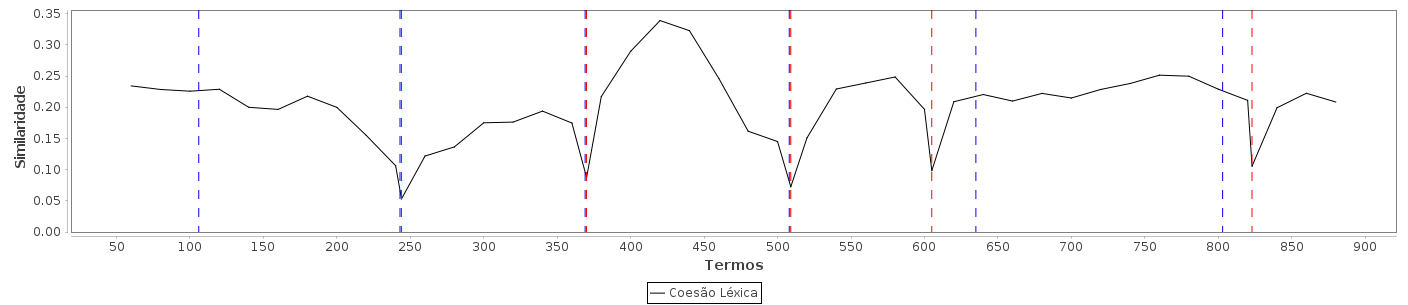
\includegraphics[width=\textwidth]{conteudo/capitulos/figs/generos-musicais-TT-40-20.png}
	  % \caption{Variação da coesão léxica ao longo de um artigo melhor estruturado em seções junto a uma segmentação automática em contraste com uma segmentação de referência.}
	  % \label{fig:coesaolexicaTT-generos-musicais}
  % \end{figure}
